%!TEX root = ../Thesis.tex
\chapter{Methodology}
This chapter describes in detail the operationalization done to answer the question of whether a \acs{SAM}-based segmentation tool can accelerate the annotation workflow of Linear A documents (see \cref{research_questions} for an overview of the individual \acsp{RQ}).
Overall, this operationalization was achieved through a comprehensive evaluation of segmentation quality (see \cref{Segmentation quality}), and a case study involving Dr. Ester Salgarella measuring the interaction efficiency (see \cref{Interaction efficiency}) and workflow efficiency (see \cref{Workflow efficiency}) of a self-developed \acs{SAM}-based segmentation tool.
In that way, these three abstract virtues were decomposed into independent measurable metrics, making it possible to concretely answer the research questions, and where the potential benefits and drawbacks of \acs{SAM} lie.
\subsection{Development environment and tools}

All software written and data collected for this thesis was made publicly available on GitHub \parencite{source_code}.
Python 3.13 was used for all code development except frontend.
The choice of this programming language was made primarily due to it being the language of choice for the \acs{ML} and \acs{SAM} implementation libraries needed.
Its big community, and library support, and package manager (pip) also made it exceptionally easy to install and manage dependencies, when seeting up the development environment.
The particular version was chosen, as it was the second latest stable release at the time of development, with the risk of Python 3.14 still not having full support by all libraries.

\section{Non-interactive segmentation} \label{Segmentation quality}
To answer the question of \hyperref[rq1]{\acs{RQ}1}: \textit{How does the initial segmentation quality of SAM compare to that of classic segmentation methods?}, the initial fully-automatic segmentation quality of \acs{SAM} was evaluated against a set of classical baseline models, using a suitable segmentation metric (i.e. \acs{Dice} score) computed from the pairs of predicted and ground truth masks.
All models were tuned through hyperparameter optimization (see \cref{subsubsec:hyperparameter_optimization}) to their best performance on the dataset, and the best performing version of \acs{SAM} was compared against the best performing baseline model.

The following subsections give an explanation of the segmentation problem itself, and document the configuration of the baseline and state-of-the-art models, as well as the evaluation protocol used to answer RQ1.

\subsection{The problem in mathematical terms}

The task of extracting the foreground (engraving and outline) from the background of an image of a writing support can be conceptualized as a binary image segmentation and classification problem at the pixel level, where each pixel is classified as either belonging to the foreground or the background.
Although this segmentation is binary, it is single-class in the sense that all foreground pixels are treated as a single foreground class, without distinguishing between different types of foreground, like tablet outlines, sign types, etc.
This segmentation process can be mathematically described as a mapping that, given some predicate function $f$, and an input image $I$, produces a binary mask $B$ of the same dimensions, where each pixel value indicates whether it belongs to the foreground (by convention denoted as 1) or the background (denoted as 0):

$$ B(x,y) = \begin{cases}
    1 & \text{if } f(I,x,y) \\
    0 & \text{otherwise} \end{cases} $$ 

\noindent In a threshold-based approach for example, the predicate function can be expressed as $f(I,x,y) = I(x,y) > T$, where $T$ is the threshold value that determines the cutoff between foreground and background pixels \parencite[p.~743]{DigitalImageProcessing}.
The predicate function does not, however, have to depend only on the individual pixel value being classified.
It can for example also be defined based on an attribute computed from the global image context (see global thresholding with Otsu in \cref{subsubsec:otsu_baseline}).
Or it can be determined from the local context of each pixel's neighborhood (see local adaptive thresholding in \cref{subsubsec:gaussian_baseline}), which can be expressed by kernel convolution working on neighborhood intensities of a window $w \in \mathbb{R}^{m \times n}$ around each pixel \parencite[p.~157,159]{DigitalImageProcessing} (where $a=(m-1)/2$ and $b=(n-1)/2$ are the vertical and horizontal half-widths of $w$, respectively, assuming odd dimensions):

$$ (w * I)(x,y) = \sum_{i=-a}^{a} \sum_{j=-b}^{b} w(i,j) I(x-i, y-j) $$

\noindent Even the entire image including external guidance can be given as context, as in the case of \acs{SAM} (see \cref{subsubsec:SAM_architecture}), where the inner workings of its transformer-based structure can be understood as a learned, non-linear black-box function that takes both image and prompts to produce the binary output mask.
Thus, the segmentation problem can evidently be approached by many different methods, each with their own contextual arguments and inner workings $f$.
And of those evaluated, it was just a matter of choosing the best one (for the evaluation details used to do that, see \cref{subsec:evaluation}).

\subsection{Baseline model configuration}
The classical baseline models against which \acs{SAM} was evaluated (from simplest to most advanced) were:
\begin{itemize}
    \item Global thresholding (Otsu's method)
    \item Local adaptive thresholding (Gaussian)
    \item Edge-based segmentation (Canny edge detection with region filling)
\end{itemize}
Together, they cover a range of classic segmentation techniques that might be used for binary foreground extraction.
Besides a description of the pre-filtering method used for all of them, what follows is a brief description of each of these methods, including their characteristics, how they work, and their implementation details.

\subsubsection{Bilateral pre-filtering} \label{subsubsec:bilateral_pre_filtering}
As a pre-filtering step for all the classical models, a bilateral filter \parencite[see][]{TomasiManduchi1998} was applied to the input image before feeding it to the classical methods.
In this way, more noise could be reduced while preserving engravings, as this filter is known to be effective at blurring out noise while preserving edges, thanks to its combined distance and intensity-dependent weighting.
Discretely \parencite[see][]{Pan2025InnovativeBilateral}, its output value $I_{\mathrm{bf}}(p)$ at a given two-dimensional pixel position $p$ (where $q$ is one of its neighbors within the kernel window with size $d$) can be defined as follows:
$$I_{\mathrm{bf}}(p)=
\frac{\sum_q I(q)\,W_{\mathrm{space}}(p,q)\,W_{\mathrm{color}}(p,q)}
{\sum_q W_{\mathrm{space}}(p,q)\,W_{\mathrm{color}}(p,q)}$$

\noindent Here, the spatial weight $W_{\mathrm{space}}(p,q)$ based on the distance between pixels $p$ and $q$, and the color range weight $W_{\mathrm{color}}(p,q)$  based on the intensity difference between $p$ and $q$ are respectively given by:
$$W_{\mathrm{space}}(p,q)=\exp(-\frac{\|p-q\|^2}{2\sigma_{\mathrm{space}}^2})$$
$$W_{\mathrm{color}}(p,q)=\exp(-\frac{\|I(p)-I(q)\|^2}{2\sigma_{\mathrm{color}}^2})$$

\noindent The method thus takes three hyperparameters: the kernel window diameter $d$, the spatial standard deviation $\sigma_{\mathrm{space}}$, and the intensity standard deviation $\sigma_{\mathrm{color}}$.
However, inspired by \parencite{OpenCVBilateralFilter}, it was decided to use the same $\sigma$ value for both spatial and color weights for the implementation, as this simplified the hyperparameter tuning (see \cref{subsubsec:hyperparameter_optimization}) without significantly compromising the filter's performance.

\subsubsection{Global thresholding (Otsu's method)}
\label{subsubsec:otsu_baseline}
Otsu's method is a global thresholding method that works on gray-level histograms, which was originally proposed by \textcite{Otsu1979}.
As the simplest of the baselines, it represents the minimum acceptable segmentation quality, since it only takes the global gray level distribution into account, with no assumptions about any spatial relationships between pixels.
It is therefore expected to perform poorly on images with erosion, uneven lighting, and differences in surface texture \parencite[p.~751]{DigitalImageProcessing}, which are the exact characteristics of the images to be segmented.
\vspace{1em}

Here is how it works:
First, let pixels of the raw image be divided into $L$ shades of gray $[1,2,...,L]$.
Then, let each pixel be assigned one of two classes $C_0$ and $C_1$, guided by a threshold $T$,
 where $C_0$ contains the shades $[1,2,...,T]$, and $C_1$ contains the rest $[T+1,T+2,...,L]$.
Otsu's method then works by performing an exhaustive search over all $L$ gray levels to find an optimal threshold $T^{*}$ that results in a maximum between-class variance $\sigma^2_B$:
$$ T^{*} = \underset{1 \leq T < L}{\arg \max} ~ \sigma^2_B(T) $$
The between-class variance $\sigma^2_B$ is then defined by a function of the respective total probabilities of the two classes ($\omega_0$ and $\omega_1$) and the mean gray level value per class ($\mu_0$ and $\mu_1$):
 $$ \sigma^2_B(T) = \omega_0(T) \omega_1(T) [\mu_1(T)-\mu_0(T)]^2$$

\noindent Without the bilateral pre-filter, this method has no hyperparameters.
\subsubsection{Local adaptive thresholding (Gaussian)}
\label{subsubsec:gaussian_baseline}
Local adaptive thresholding works by computing a threshold for each pixel based on its local neighborhood.
This is an advantage in cases where the image has varying light conditions (which is the case for the images to be segmented), as the threshold adapts to local lighting.

Mathematically, the local threshold $T$ is a function of a given pixel position $(x,y)$ computed by a weighted sum of the neighborhood.
The generated binary mask $B$ is then defined as \parencite[p.~761]{DigitalImageProcessing}:
$$ B(x,y) = \begin{cases}
    1 & \text{if} ~ I(x,y) > T(x,y) \\
    0 & \text{otherwise} \end{cases} $$

To compute $T(x,y)$, there are a few weighting functions to choose from.
For this baseline, the Gaussian kernel was used, as it can limit the influence of distant noisy pixels on the computed threshold by assigning weights based on distance from the kernel center.
With a Gaussian kernel  $G_{\sigma}$, the threshold $T(x,y)$ is computed as a Gaussian-weighted sum of local intensities subtracted by a constant $C$. Using kernel convolution ($*$), this can be expressed as \parencite[see][p.~761]{opencv_adaptive_threshold}:
$$ T(x,y) = (G_{\sigma} * I)(x,y) - C $$

In general, the weight in the Gaussian kernel at an offset $(i,j)$ from the kernel center can be written as follows (where $\alpha$ is a normalization constant ensuring that the whole kernel sums to 1, and $\sigma$ controls the spatial spread of the kernel) \parencite[p.~167]{DigitalImageProcessing}:
$$ G_{\sigma}(i,j) = \alpha \cdot \exp\left(-\frac{i^2 + j^2}{2\sigma^2}\right) $$

\noindent Thus, without the bilateral pre-filter, this method has two hyperparameters: the kernel size $d$, and the constant $C$.

\subsubsection{Edge-based segmentation (Canny edge detection with region filling)}
Canny edge detection is a method that by itself only segments the edges of an image, excluding the enclosed regions within those edges.
First, for the image gradient of each pixel, the magnitude $M_s(x,y)$ and the orientation $\theta_s(x,y)$ are computed \parencite[p.~730]{DigitalImageProcessing}:
$$M_s(x,y) = \|\ \nabla I_{s}(x,y) \|\ = \sqrt{\left(\frac{\partial I_{s}}{\partial x}\right)^2 + \left(\frac{\partial I_{s}}{\partial y}\right)^2}$$ 
$$\theta_s(x,y) = \arctan \left( \frac{\partial I_{s}/\partial y}{\partial I_{s}/\partial x} \right)$$
Next, \textit{non-maxima suppression} \parencite[p.~730-731]{DigitalImageProcessing} is applied to retain only local maxima of $M_s(x,y)$ along the gradient direction $\theta_s(x,y)$, resulting in thinner edges.
This is then followed by \textit{hysteresis thresholding} \parencite[p.~732]{DigitalImageProcessing}, classifying pixels as strong, weak, or non-edges with a low threshold $T_l$ and a high threshold $T_h$, only preserving weak edges if connected to strong edges.

Inspired by \parencite{autocanny}, for the implementation, these thresholds were automatically determined by introducing a hyperparameter $\sigma$ that controls the sensitivity of the edge detection (where $v$ is the median of the grayscale values of the given image):
$$
T_l = \max\bigl(0, (1 - \sigma)\, v\bigr), \quad
T_h = \min\bigl(255, (1 + \sigma)\, v\bigr)
$$

\noindent Then, in an attempt to fill the regions enclosed by the detected edges, morphological closing (dilation followed by erosion) was applied to the edge mask.

Hence, without the bilateral pre-filter, this method has two hyperparameters: the constant $\sigma$, and the kernel size $d$ used for morphological closing.

\subsection{State-of-the-art}
To be compared against the classical baselines was the generalized deep learning \acf{SAM} \parencite{sam}.
Due to its popularity as a \acs{SOTA} segmentation model, and the fact that its different use cases require different trade-offs in terms of accuracy, speed, and domain adaptation, there are many different variants of \acs{SAM}.
For the sake of fairness, it seemed only reasonable to test out the following range of them:\footnote{Due to access restrictions of the checkpoints (weight files) necessary for running the newly released \acs{SAM}3 \parencite{sam3}, it was not included in the evaluation.}
\begin{itemize}
    \item The original \acs{SAM} \parencite[see][]{sam}, and its computationally efficient variant Mobile\acs{SAM} \parencite[see][]{mobile_sam_v2}
    \item The newer \acs{SAM}2 \parencite[see][]{sam2}
    \item The few-shot variant \acs{FATESAM} \parencite[see][]{fatesam} and one-shot variant \acs{GFSAM} \parencite[see][]{gfsam}
\end{itemize}

\noindent Together, these variants span the axes of relevance, recency and \acs{ICL} capabilities that should make for a fair test.

Furthermore, for additional fairness, a small ablation study was conducted on the base models (\acs{SAM}, Mobile\acs{SAM}, \acs{SAM}2) to investigate whether these variants benefitted from the use of bilateral pre-filtering (see \cref{subsubsec:bilateral_pre_filtering}), and automatic threshold-derived point prompts (see \cref{subsubsec:automatic_prompts}).

To be able to run all these computationally demanding variants of \acs{SAM}, model execution was outsourced to Modal \parencite[see][]{modal_docs} -- a serverless cloud computing platform usually used for \acs{ML} inference, tuning and training.
The following subsections describe the architecture of the chosen variants, and how they were implemented in the evaluation.

\subsubsection{SAM architecture}
\label{subsubsec:SAM_architecture}
Used by \acs{SAM} and Mobile\acs{SAM}, the first \acs{SAM} model architecture released \parencite{sam} consists of an image encoder, and a comparatively lightweight prompt-guided mask decoder (see \cref{fig:SAM_architecture}).
This image encoder takes the form of a \acf{ViT}, that similarly to a \acf{CNN} processes an input image in order to extract its features \parencite{imageworth16x16words}.
Instead of relying on just convolutional layers, however, a \acs{ViT} adapts the transformer architecture originally developed for \acs{NLP} to the image domain.
Rather than words, an image is treated as a sequence of fixed-size patches (regions of the image), each of which is embedded into a vector representation and augmented with a positional encoding, analogous to how tokens are handled in \acs{NLP}.
Seen in \cref{fig:ViT_architecture}, these embedded patches are then passed through a repeated layered series of normalization, learned feed-forward \acfp{MLP}, and, in between, a learned mechanism known as self-attention that weighs the embeddings according to their relevance to one another.
\begin{figure}[htp]
\centering
    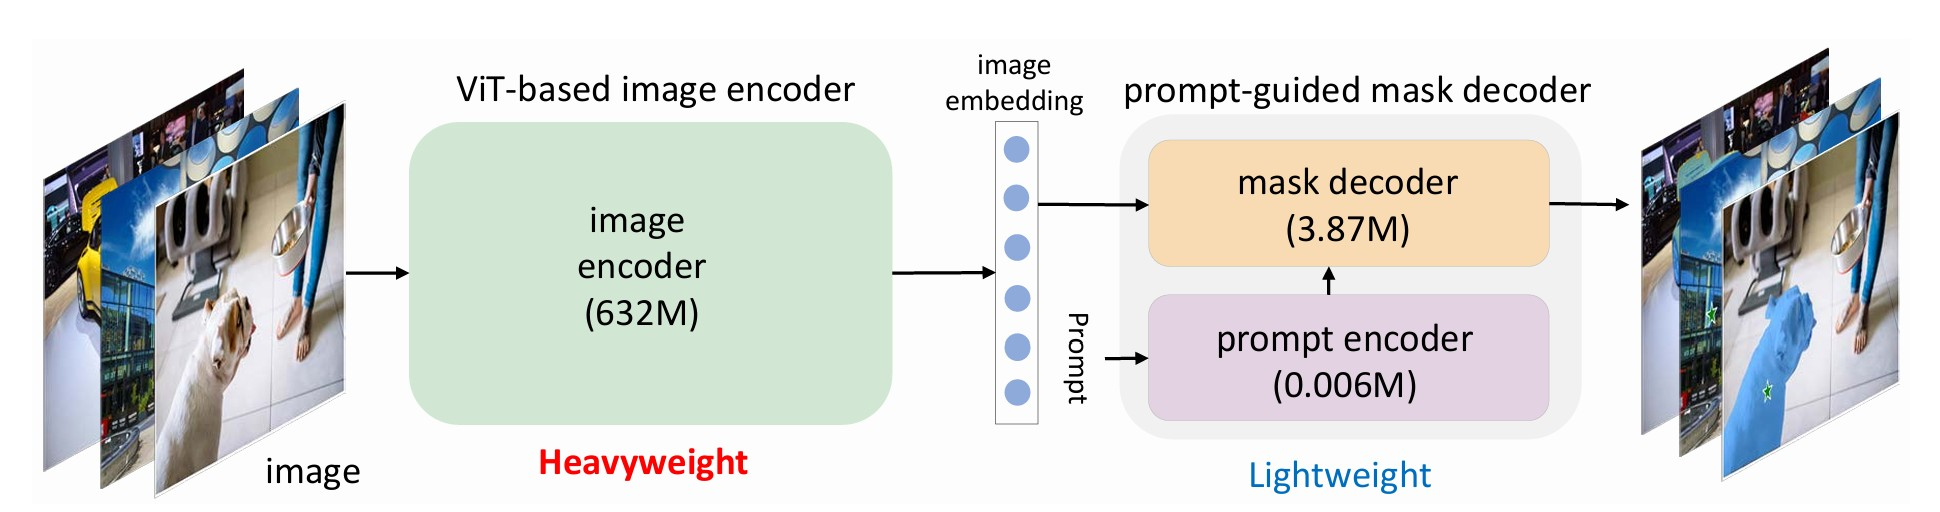
\includegraphics[width=\linewidth]{images/SAM-architecture.jpg}
\caption{Architecture of \acs{SAM}, from \textcite{mobile_sam}.
An input image is processed by a \acs{ViT}-based image encoder to produce an image embedding, which is then fed to a comparatively lightweight (also transformer-based) prompt-guided mask decoder along with embedded prompts to generate the final segmentation mask.}
\label{fig:SAM_architecture}
\end{figure}

\begin{figure}[htp]
\centering
    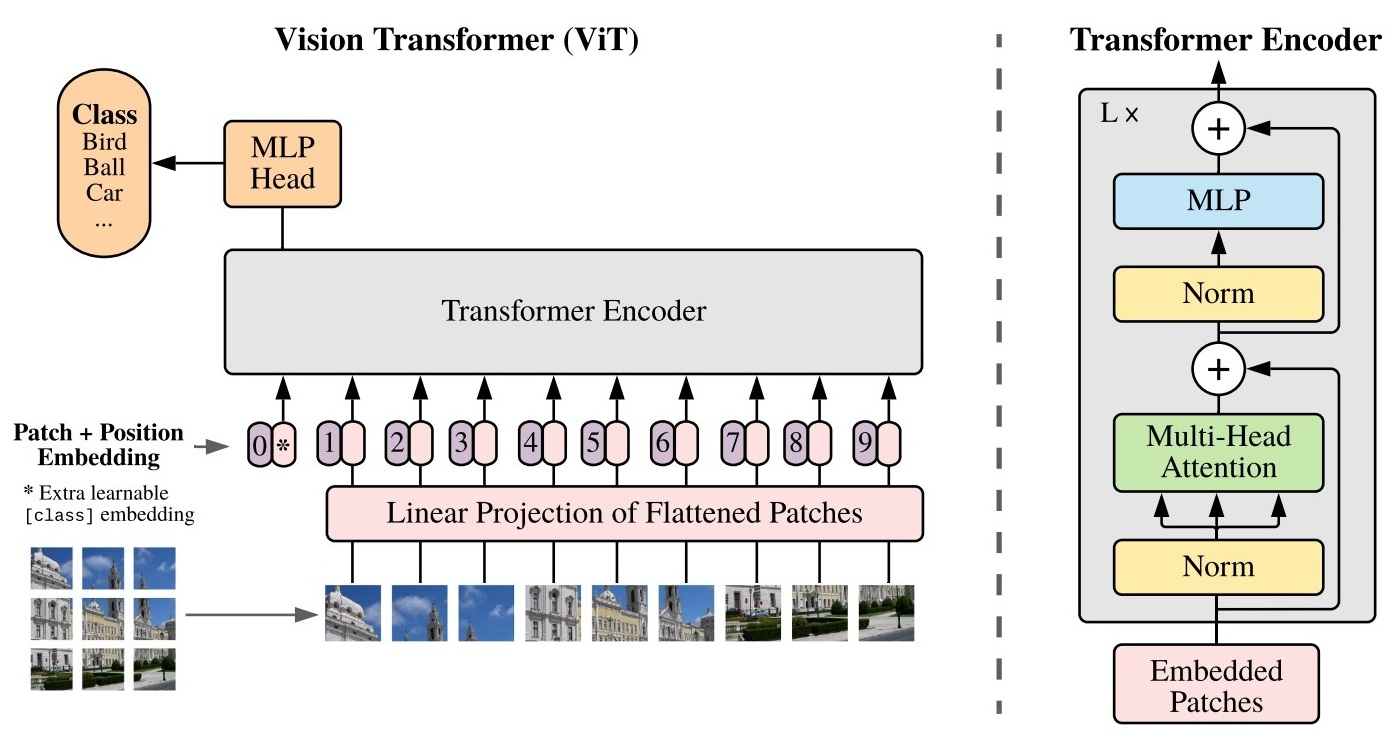
\includegraphics[width=\linewidth]{images/ViT-architecture.jpg}
\caption{Architecture of the \acs{ViT}, from \textcite{imageworth16x16words}.
An image is treated as a sequence of flattened fixed-size patches, each embedded into a vector representation augmented with a positional encoding.
These embeddings are then passed through a repeated layered series of normalization, learned feed-forward \acfp{MLP}, and learned self-attention.}
\label{fig:ViT_architecture}
\end{figure}

More specifically \parencite[according to][]{vaswani2023attentionneed}, given an input embedding $X$, self-attention computes three projections; the queries $Q$, keys $K$, and values $V$, as products of $X$ with their respective learned matrices, and passes the information on as a new matrix (where $d_k$ is the dimension of $Q$ and $K$):
$$ \mathrm{Attention}(Q,K,V) = \mathrm{softmax}\left(\frac{QK^T}{\sqrt{d_k}}\right)V $$
Here, the $\mathrm{softmax}$ normalization function turns the scaled query--key similarities $\frac{QK^T}{\sqrt{d_k}}$ into a set of attention weights (each on the interval $]0, 1[$, in total summing to 1), which determine how the value vectors $V$ are combined into the input of the next layer.

Finally, the \acs{ViT} outputs an image embedding that captures the spatial context of the image.
It is this image embedding, combined with embedded prompts from the prompt encoder (referred to as prompt tokens), that is fed to the mask decoder in order to generate the final segmentation mask.
Before this can happen, however, the prompt encoder must convert any given sparse prompts (i.e. box or point prompts) into embeddings, which is done by summing their positional encodings with learned type-specific embeddings (one foreground/background embedding per point prompt, and two opposite-corner embeddings per box prompt).

Seen in \cref{fig:SAM_mask_decoder}, these are then fed to the lightweight mask decoder (which is also transformer-based) along with the image-embedding from the \acs{ViT}, and three learnable output token embeddings (see \cref{fig:SAM_mask_decoder}).
However, for a generation of single output masks, which is what was used in this thesis for all models except \acs{GFSAM}, the mask is generated from just a single output token \parencite[p. 17]{sam}, 

Self-attention is then applied to the prompt and output tokens, and two-way cross-attention (same as self-attention but with one embedding as queries, and the other as keys and values, and vice-versa) is applied between the tokens and image embedding for them to influence and attend one another.
To keep track of spatial coordinates and prompts, the image embedding, and the original prompt embeddings along with their positional encodings are added as input at every attention layer.

\begin{figure}[htp]
\centering
    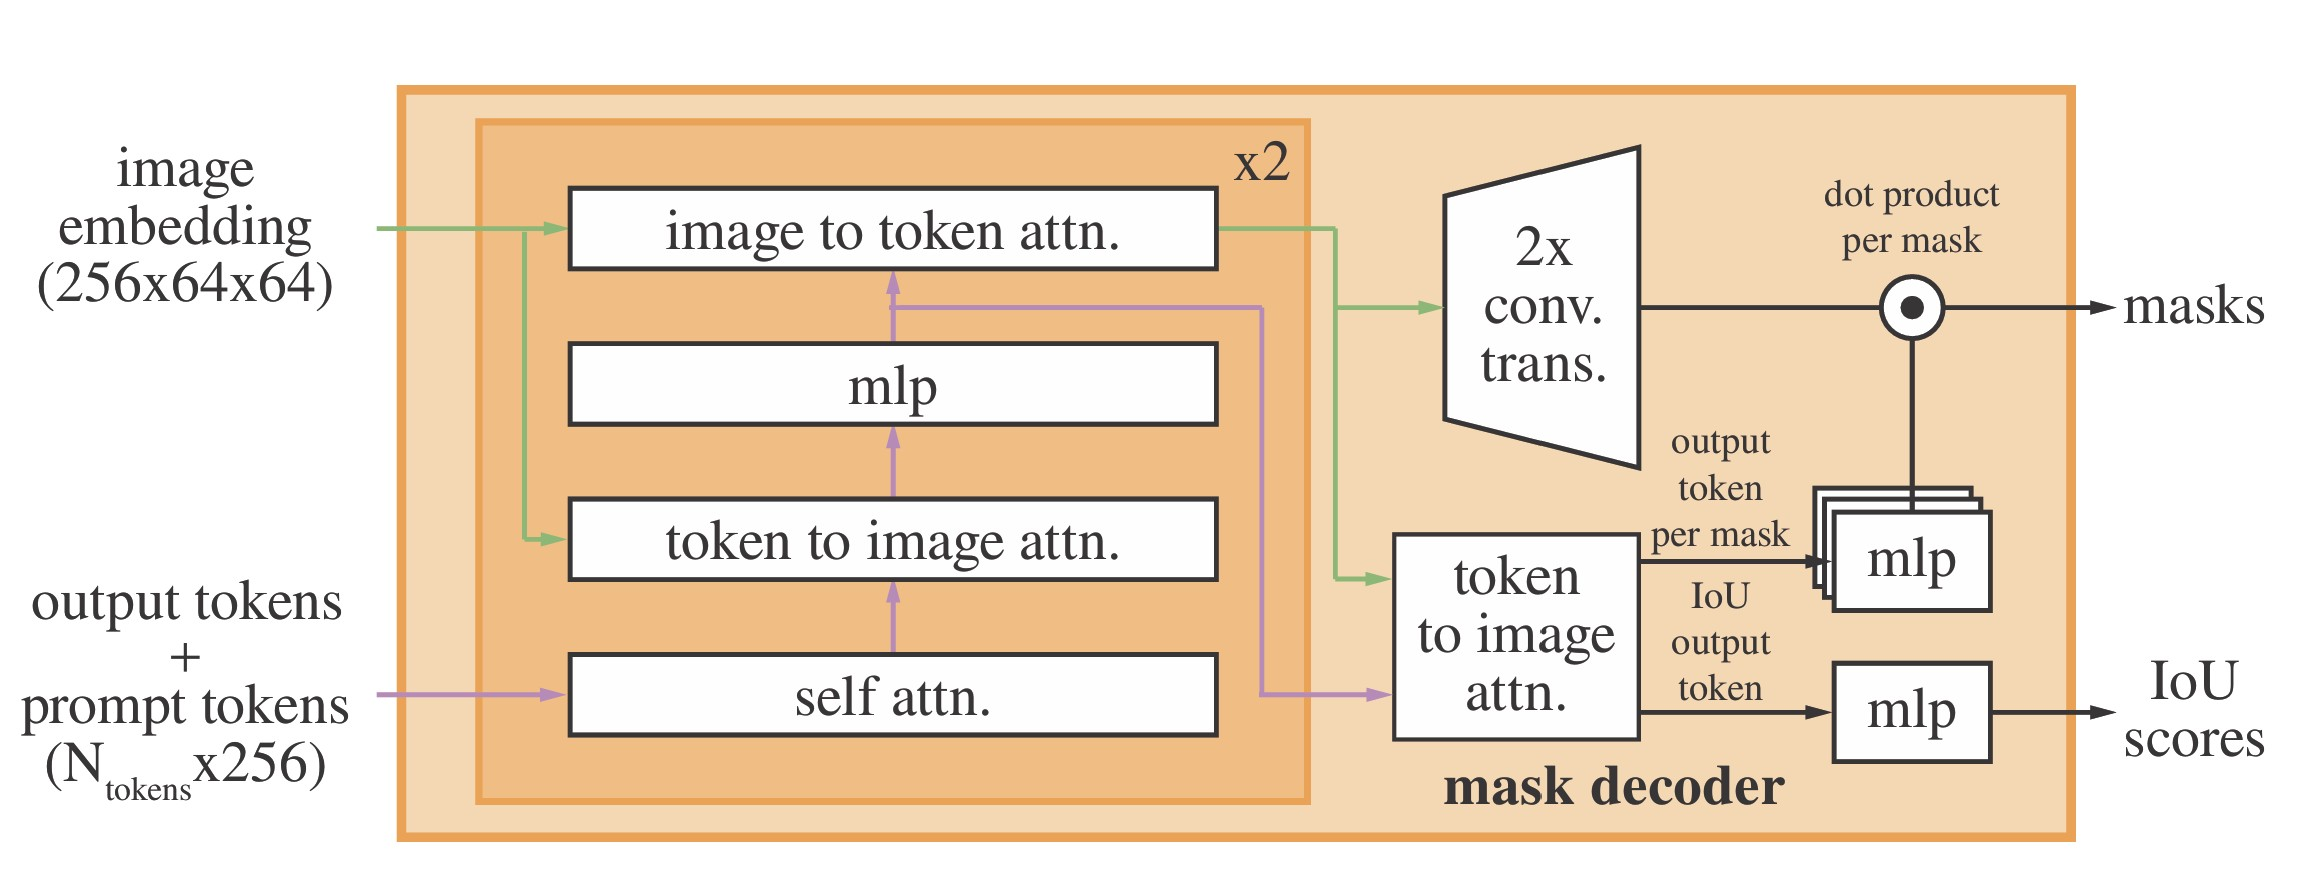
\includegraphics[width=\linewidth]{images/SAM-mask-decoder.jpg}
\caption{Architecture of \acs{SAM}'s mask decoder, from \textcite{sam}.
The image embedding, embedded prompts, and learnable output tokens interact through self-attention and two-way cross-attention, after which the image embedding is upsampled by convolution and the output tokens are processed by two types of \acsp{MLP}: one whose output is combined with the upsampled image embedding via a dot product to generate the segmentation masks, and another that outputs a predicted IoU score per mask.}
\label{fig:SAM_mask_decoder}
\end{figure}

At the end of this process, the image embedding is upsampled by convolution to the original image resolution.
The output tokens are then processed in parallel by two types of \acsp{MLP}:
one that generates the final segmentation masks by taking a dot product between each token and the upscaled image embedding,
and another that outputs a predicted IoU score for each mask.

For the implementation of \acs{SAM} in the evaluation, the ViT-H checkpoint was used, as it is the largest and best-performing of the available variants.
Mobile\acs{SAM}, by definition, instead relied on the lighter \acs{ViT} variant TinyViT \parencite{TinyViT}, whose 5M parameters are far fewer than those of the \acs{SAM} encoders (ViT-H, ViT-L, and ViT-B, with 632M, 307M, and 86M parameters, respectively).
It is this reduction in encoder size that makes Mobile\acs{SAM} computationally faster than the original.

\subsubsection{SAM2}

With the release of \acs{SAM}2 \parencite{sam2}, the image encoder was changed to Hiera \parencite{hiera} -- a hierarchical \acs{ViT}, which by lowering attention complexity is more parameter efficient than vanilla \acs{ViT}s, as tokens are pooled together at different stages of the encoding process. 
Additionally, a memory attention mechanism was added for consistency, allowing the model to attend to segmentation outputs of previous frames to make masks between frames consistent enough to segment videos.
As seen in \cref{fig:SAM2_architecture}, it does so by storing a memory-encoded version of the mask output of each previous frame in a memory bank that are then attended to by the image-encoded embeddings before being passed to the mask decoder.
\begin{figure}[htp]
\centering
    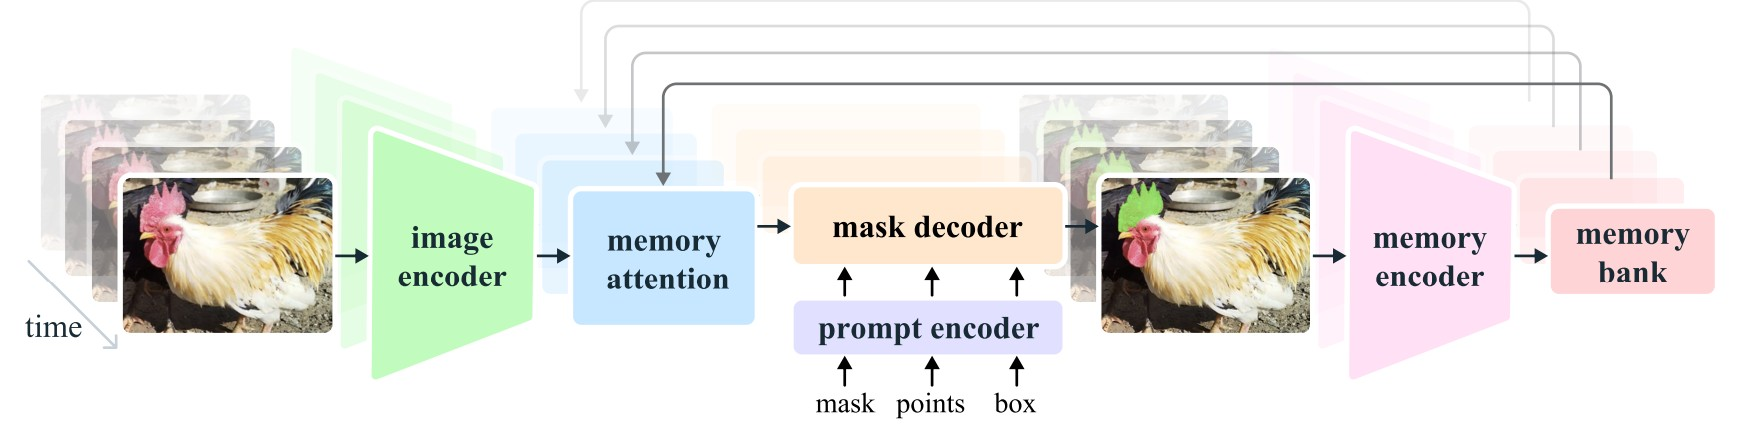
\includegraphics[width=\linewidth]{images/SAM2-architecture.jpg}
\caption{Architecture of \acs{SAM}2, from \textcite{sam2}.
A learned memory attention mechanism was added, allowing the model to segment videos.
For each frame, the output mask is encoded by a learned memory encoder and stored in a memory bank, whose contents are attended to by the image-encoded embeddings before being passed to the mask decoder.}
\label{fig:SAM2_architecture}
\end{figure}

\acs{SAM}2 was pre-trained on both still images and video, first on the \acs{SA-1B} image dataset \parencite{sam} and then on the \acf{SA-V} dataset \parencite{sam2}.
The mask decoder did not change much from the original (\cref{fig:SAM_mask_decoder}), except for the passing of early visual features from the Hiera image encoder to the convolutional upsampling process, improving the integrity of the output mask.
But also added were object pointers as lightweight vectors keeping track of the semantic information of each object of interest.
These are also stored in the memory bank together with the spatial memory, and attended to in memory attention.

As for the implementation of \acs{SAM}2 in the evaluation, the checkpoint chosen was \texttt{sam2.1\_hiera\_large}, as it was the best performing one listed in the repository of \acs{SAM}2 \parencite{sam2_repo}.
\acs{SAM}2 also takes a checkpoint-specific YAML configuration file, which stores the hyperparameters for the model, and allows for easy overrides through Hydra.
Since the tablets were segmented as individual still images, \acs{SAM}2's image predictor was used rather than the video predictor.
The memory and video-tracking machinery is only relevant to the \acs{FATESAM} adaptation described in the next section.

\subsubsection{FATESAM} \label{subsubsec:FATESAM}
Within the domain of 3D medical images, \acs{FATESAM} -- a training-free few-shot adaptation of \acs{SAM}2 \parencite[see][]{fatesam} has been recently demonstrated to surpass even the best fine-tuned versions of \acs{SAM}.
As seen in \cref{fig:FATESAM_architecture}, it works in principle by making use of \acs{SAM}2's architecture and memory attention mechanism, by passing a few support images to its memory encoder, such that the mask decoder ends up with context to generate a similar segmentation mask for the input query image.

At inference of the 2D-adaptation made, support masks $y_s^{j}$ (rather than support mask volumes $y_s^{ij}$ with index slice $i$) are chosen by the similarity of their corresponding image-encoded support images $\mathcal{E}(x_s^{j})$ to the image-encoded query image $\mathcal{E}(x)$ to make sure that they are as representative as possible.
Like the original, this ranking is computed ascendingly from the Manhattan distances between the image-encoded features of the input and the support images.
As memory encoded embeddings $\mathcal{ME}(y_s^{j})$, these support masks are then passed to memory attention $\mathcal{MA}$ together with the image-encoded query image $\mathcal{E}(x)$, whereafter the output is passed on to the mask decoder $\mathcal{D}$ to generate the final mask ${y}$.

\begin{figure}[htp]
\centering
    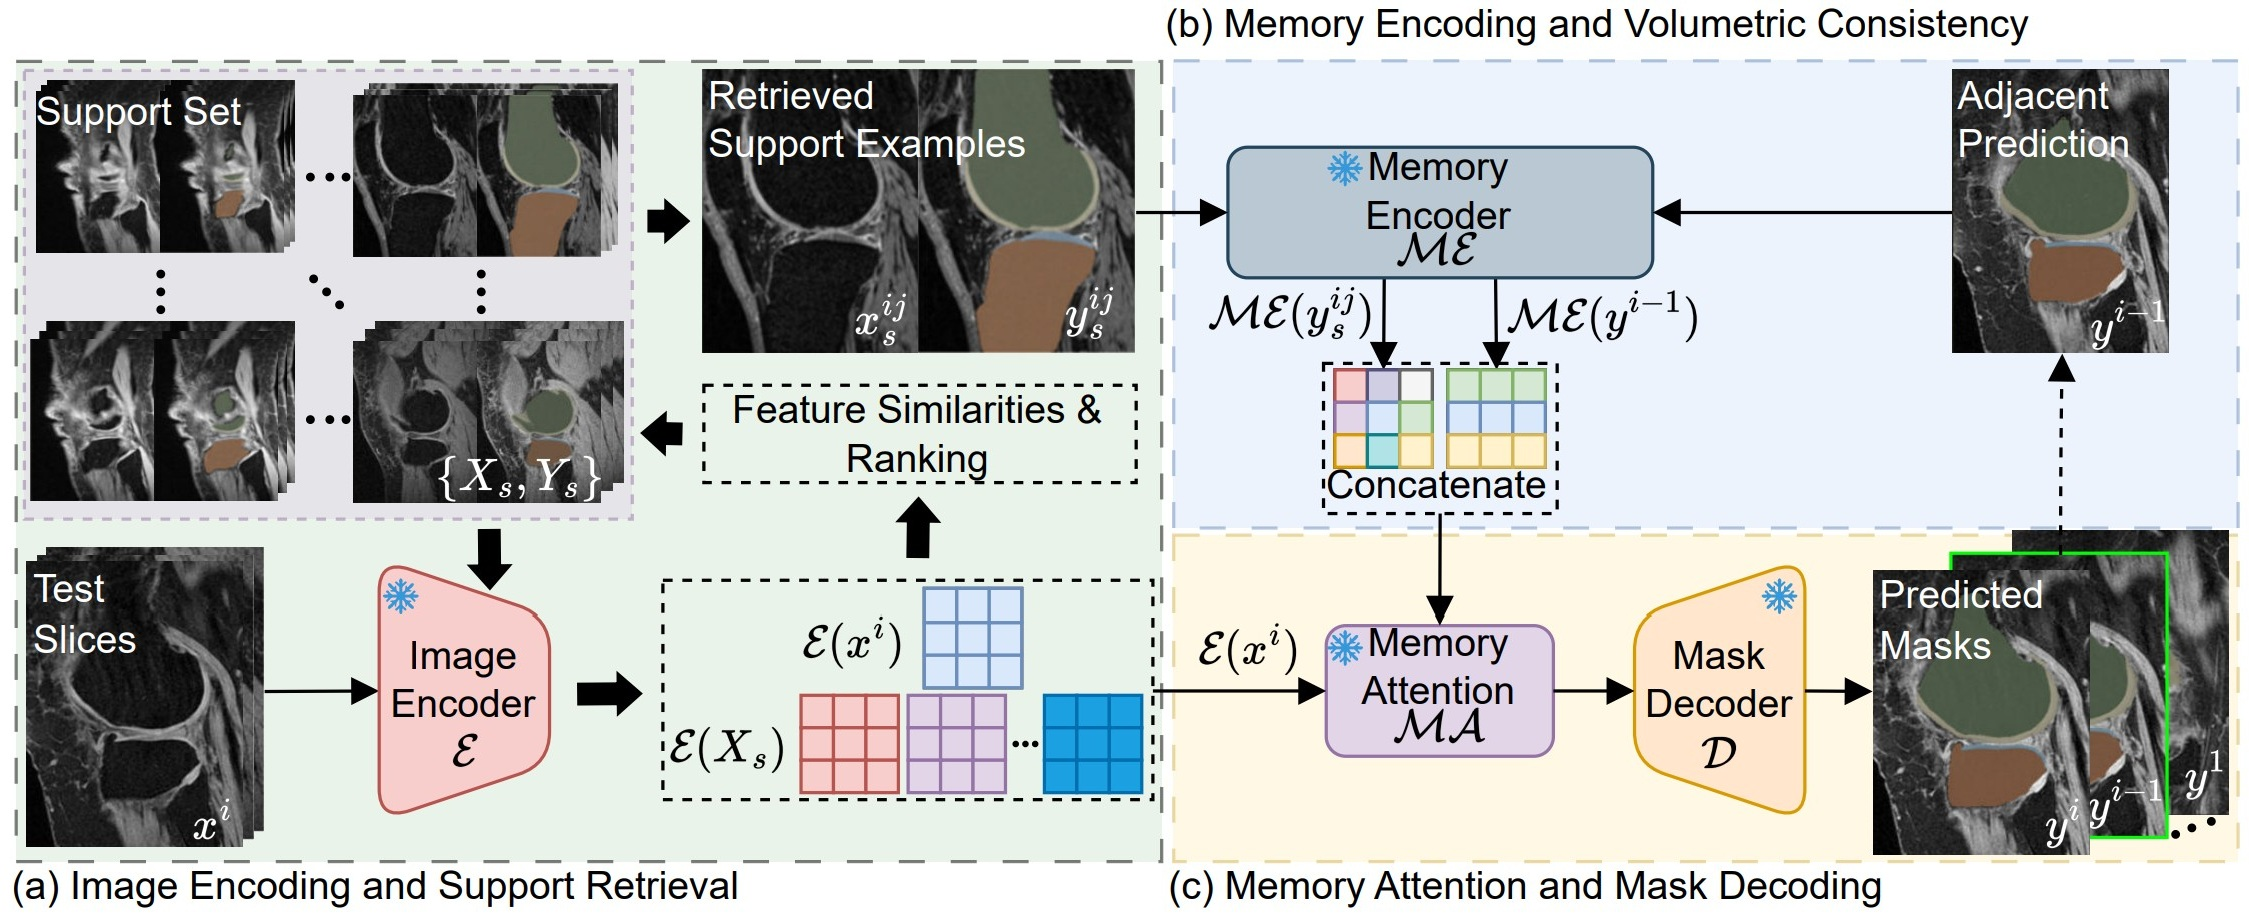
\includegraphics[width=\linewidth]{images/FATESAM-architecture.jpg}
\caption{Architecture of \acs{FATESAM}, from \textcite{fatesam}.
At inference of the 2D-adaptation, support masks $y_s^{j}$ are first chosen (a) by the similarity of their corresponding image-encoded support images $\mathcal{E}(x_s^{j})$ to the image-encoded query image $\mathcal{E}(x)$ and then passed (b,c) to memory attention $\mathcal{MA}$ as memory encoded embeddings $\mathcal{ME}(y_s^{j})$.
Unlike the original's 3D inference, no adjacent
predictions $y^{i-1}$ are relevant, since a Linear A image is
treated as an independent 2D input frame $x$.}
\label{fig:FATESAM_architecture}
\end{figure}

The adaptation of \acs{FATESAM} in the evaluation was based on the official repository \parencite{fatesam_repo}, and the checkpoint used was \texttt{sam2\_hiera\_large}, as it was the best performing one used by the repository.
Three support images were injected per query image, as this was the number of support units that was found to be most optimal in the paper \parencite{fatesam}.
To further adapt \acs{FATESAM} to single frame images, the object pointer functionality was turned off through Hydra/YAML overrides, which was necessary to avoid shape mismatches.
In particular, the object-pointer encoder and object-score prediction heads were disabled by setting
\texttt{use\_obj\_ptrs\_in\_encoder},
\texttt{pred\_obj\_scores},
\texttt{pred\_obj\_scores\_mlp}, and 
\texttt{fixed\_no\_obj\_ptr} all to false.
Attempts were made to contact the authors of \acs{FATESAM} about the correctness of this adaptation, but no response was received.
Interestingly, in the ablation study of object pointers in \acs{SAM}2 \parencite[see][p. 15]{sam2}, its importance was only evaluated on video datasets and included on that basis.
It was hence deemed reasonable to assume that it would not contribute to the performance of \acs{FATESAM} on single frame images, and thus could be turned off without compromising performance.

\subsubsection{GFSAM} \label{subsubsec:GFSAM}
The other kind of training-free \acs{ICL} adaptation of \acs{SAM} tested was the one-shot \acs{GFSAM} \parencite[see][]{gfsam}.
As seen in \cref{fig:GFSAM_architecture}, it works by first extracting the features of the given support image and the query image by using the pre-trained image encoder DINOv2 \parencite{dinov2}.

With its Positive-Negative Alignment module, \acs{GFSAM} then computes two similarity maps between query and support features: one for positive/object similarity, and one for negative/background similarity.
These maps are used to generate foreground point prompts for \acs{SAM}, which are then fed to the mask decoder that generates one mask per point prompt.
A graph is then constructed of the coverage of the points lying within each of the generated masks, whereafter the removal of some of the points representing weakly connected components is determined through processes referred to as Positive Gating and Overshooting Gating.
The purpose of those gating processes is to filter out false-positive masks, where the former process makes sure a given point is actually foreground according to the similarity maps, and the latter ensures that the point is not a boundary-near outlier.
Finally, the masks associated with the remaining points are merged together to generate the final mask.
If instead no points remain after the gating processes, the mask with the highest predicted IoU score is selected as the final mask.
\begin{figure}[htp]
\centering
    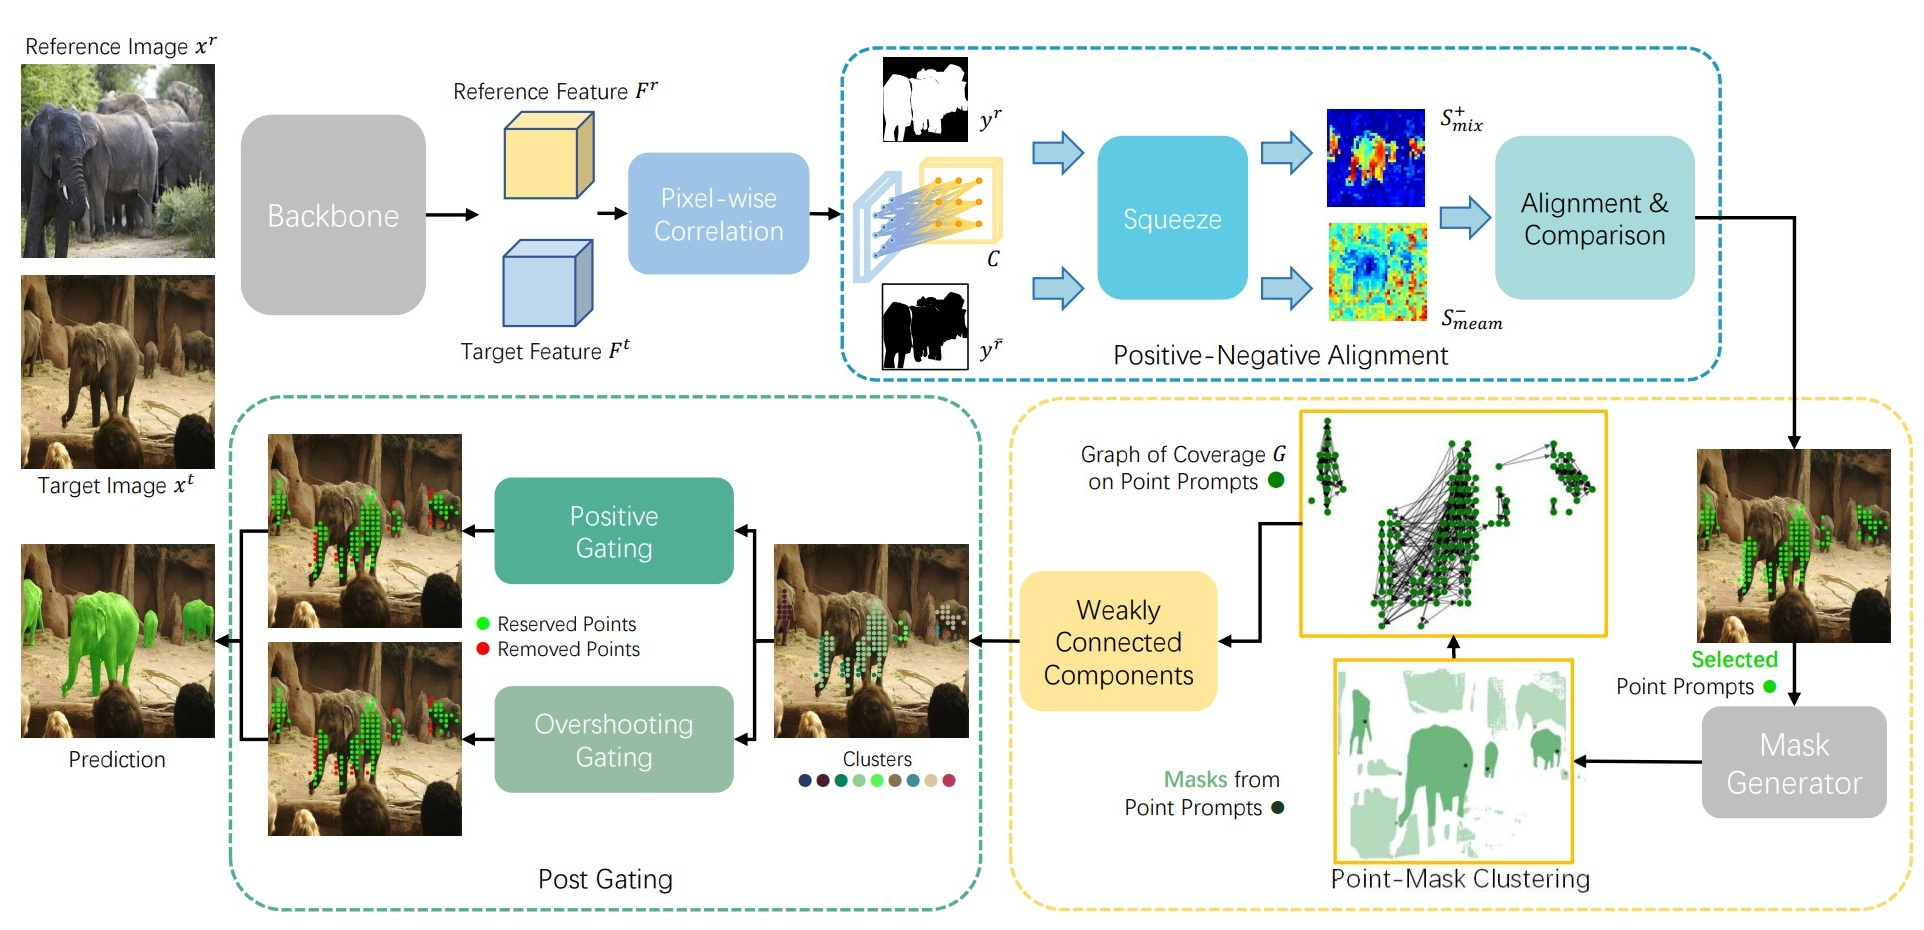
\includegraphics[width=\linewidth]{images/GFSAM-architecture.jpg}
\caption{Architecture of \acs{GFSAM}, from \textcite{gfsam}.
Features of the one-shot support and query images are first extracted with the pre-trained DINOv2 encoder, from which the Positive-Negative Alignment module computes object- and background-similarity maps.
These maps give rise to foreground point prompts for \acs{SAM}, which generates one mask per point.
 A graph of the points' coverage within each of these masks then removes weakly connected, false-positive points via Positive and Overshooting Gating, whereafter the masks of the surviving points are merged into the final segmentation mask.}
\label{fig:GFSAM_architecture}
\end{figure}

The implementation of \acs{GFSAM} in the evaluation was based on the official repository \parencite{GFSAMRepository} with its DINOv2 feature encoder using the ViT-L/14 checkpoint, and \acs{SAM} using the ViT-H checkpoint.
As an adaptation to the data domain, the one-shot support image was selected in the same way as for \acs{FATESAM}: the support images were ranked by the Manhattan distance of their DINOv2 features to those of the query image, and the most similar one was selected as support.

\subsubsection{Threshold-inferred automatic point prompts}
\label{subsubsec:automatic_prompts}
Another way to adapt \acs{SAM} to the specific characteristics of the domain was through the use of automatic prompts.
As it is particularly difficult to automatically create meaningful box prompts without a trained object detection model, only point prompts were used for this adaptation.

\noindent Inspired by \acf{POI} placement in \parencite{promptSAM}, automatic point prompts for \acs{SAM} were derived from the output mask of the Gaussian thresholding baseline (see \cref{subsubsec:gaussian_baseline}).
This was done by randomly sampling a number of foreground and background pixels from the classical output mask as prompts for \acs{SAM}.
Concretely, $n_{fgd}$ foreground points and $n_{bgd}$ background points were sampled from the foreground and the eroded background of the mask, respectively (see \cref{fig:autoprompt_SAM} for a visual example).
Without the hyperparameters of \acs{Gaussian}, this method thus introduces three hyperparameters: $n_{fgd}$, $n_{bgd}$, and the erosion kernel size $d$.

\begin{figure}[htp]
\centering
    \fbox{\includegraphics[width=0.4\linewidth]{../src/data/results/autoprompt_displays/\exampleTabletName-SAM+pts-no-filter.jpg}}
\caption{A visual example of prompt distribution for the \acs{POI} prompt strategy, overlaid on \displayexampleTabletName.
Green points represent foreground point prompts, while red points represent background point prompts.}
\label{fig:autoprompt_SAM}
\end{figure}


\subsection{Evaluation protocol for \acs{RQ}1}
\label{subsec:evaluation}
To determine whether one model performed significantly better than another, a relevant metric (\acs{Dice}) and a statistical test (paired t-test) needed to be defined.
Additionally, to ensure a fair comparison, all models with hyperparameters were optimized to their best performance on the validation set.
What follows is a description of this evaluation protocol.

\subsubsection{Choice of metric (\acs{Dice})}
\label{subsubsec:metrics}
When it comes to evaluation of segmentation models, the two most commonly used metrics are the \acf{Dice} and the \acf{IoU}. The \acs{Dice} score is most commonly used in cases where there are heavy class imbalances (e.g. lots of background compared to regions segmented), and when foreground objects are small and thin.
It is naturally more forgiving than the related segmentation metric \acs{IoU}, which is more strict and specifically used to evaluate segmentation results where small displacements are critical for results.
Therefore, segmentation performance was reported using \acs{Dice}. Mathematically, it is defined as twice the size of the intersection of the predicted segmentation mask $\hat{Y}$ and the ground truth mask $Y$, divided by their summed size \parencite{Metrics2025}:

$$ \mathrm{Dice}(\hat{Y}, Y) = \frac{2 \cdot | \hat{Y} \cap Y |}{|\hat{Y}| + |Y|} $$

\noindent The raw metrics thus ended up consisting of \acs{Dice} scores produced per image for each model.

\subsubsection{Hyperparameter optimization (\acs{TPE})}
\label{subsubsec:hyperparameter_optimization}
All models with hyperparameters were tuned to their best \acs{Dice} scores on the validation set (see \cref{sec:dataset}) in a series of 100 trials each using Optuna \parencite{optuna2019}, a hyperparameter optimization framework.
The optimization itself was performed using the \acf{TPE} algorithm \parencite{TPEHyperparameterOptimization2013,TPEHyperparameterOptimization2011},
which is a Bayesian optimization method that models the relationship between hyperparameters and performance to efficiently explore the hyperparameter space and find the optimal ones.
Hence, it is more sophisticated than a random search, which just samples different hyperparameter combinations without considering the results of past evaluations.

It works by building two probabilistic models: one for the configurations that have resulted in good performance, and another for those that have resulted in poor performance.
It then uses these models to select the next hyperparameter configuration to evaluate, selecting the one that maximizes the expected improvement.
This way, it can focus the search on promising regions of the space of possible hyperparameters, removing the need to rely on chance or exhaustive search.


\subsubsection{Statistical test (paired t-test)}
To determine whether the observed difference in \acs{Dice} scores between the two strongest models was statistically significant, a paired t-test was conducted.
Specifically, a one-tailed paired t-test was used, as the alternative hypothesis was that \acs{SAM} would perform significantly better than the best classical baseline, instead of just significantly differently.
The paired t-test has two main assumptions: 1. independence of tested observations, and 2. normality of the paired differences.
The first assumption is already satisfied a priori, since the segmentation performance of one image does not directly influence the performance on another.
However, the second assumption depends on the results.
Thus, the paired differences in \acs{Dice} scores between the two models tested needed to be checked for normality using a QQ-plot and the Shapiro-Wilk test.
In case the normality assumption was violated, the non-parametric domain-specific Wilcoxon signed-rank test would be used instead \parencite{Rainio2024}.


\section{Tool-side interaction} \label{Interaction efficiency}
To answer the question of \hyperref[rq2]{\acs{RQ}2}: \textit{To what extent can user interaction be reduced by a \acs{SAM}-based semi-automatic segmentation workflow, while still maintaining high-quality outputs?}, a two-in-one interactive segmentation tool was developed including a method meant to represent \acs{SAM}, and another to represent the classical segmentation methods, to allow for a direct comparison in terms of tool efficiency.
The following subsections go into details on how this tool was developed, the experimental design for the evaluation of interaction efficiency, and the definition of interaction metrics.
\subsection{Tool development}
The tool was developed in close collaboration with Ester Salgarella, in an attempt to make it fit her workflow and needs as much as possible.
However, before any user tests were conducted, a \acf{MVP} was developed based on the workflow that she had described throughout the fortnightly supervisor meetings attended during the writing of this Thesis from February 2nd 2026, and the few sporadic meetings and written exchanges since November 2025 that took place during the planning of the project proposal.
When this \acs{MVP} was ready, three usability tests were conducted with Ester, two of them online, and the last one in-person at \acf{AIAS}.

During these usability tests, Ester was asked to perform the segmentation of at least one document with each method of the tool, while thinking aloud and giving feedback on the user experience.
Small modifications were then made to the tool based on her feedback, until the final acceptance test was conducted.
These tests took place the 5th, 8th and 12th of May (see \cref{appendix:usability-tests} for documentation).



\subsection{Tool architecture}
The architecture of the tool (see \cref{fig:tool-architecture}) was developed as a web-application using Svelte as the frontend framework, and FastAPI as the backend framework, hosted via Render \parencite{Render}.
Because it was made a web application, it could be run remotely on any device through a web browser, without the need for installation, making it more easily accessible and ideal for online user testing with Ester Salgarella.
To make the development environment more consistent with production, the application was containerized using Docker, which made it easier to deploy and run on any machine without worrying about dependencies and environment setup.

Svelte was chosen for the frontend mostly due to its reactive state management, making it well-suited for building interactive user interfaces, as this functionality removes the need for re-inserting state variables every time they change.
FastAPI was chosen as the backend, as it is Python based, and therefore able to serve the Python segmentation models implemented, which was essential for the tool's functionality.
It is also lightweight and asynchronous, which potentially allowed for many users to use the tool simultaneously, as several requests could be handled at the same time without blocking execution on the server.

\begin{figure}[htbp]
\centering
\begin{tikzpicture}[
    node distance=1.8cm,
    component/.style={
        rectangle,
        rounded corners,
        draw,
        align=center,
        minimum width=6.4cm,
        minimum height=1.15cm,
        inner xsep=4pt,
        inner ysep=3pt
    },
    logo/.style={
        inner sep=0pt
    },
    arrow/.style={-{Latex}, thick}
]

% Main modules
\node[component] (svelte) {
    Svelte frontend\\
    \footnotesize browser interface, preview, export
};

\node[component, below=of svelte] (fastapi) {
    FastAPI backend\\
    \footnotesize segmentation API, OpenCV methods
};

\node[component, below=of fastapi] (modal) {
    Modal cloud service\\
    \footnotesize GPU-based SAM inference
};

% Hovering logos to the left
\node[logo, left=0.4cm of svelte] {
    
\includegraphics[width=0.75cm,height=0.75cm,keepaspectratio]{images/Svelte.png}
};

\node[logo, left=0.4cm of fastapi] {
    
\includegraphics[width=0.75cm,height=0.75cm,keepaspectratio]{images/FastAPI.png}
};

\node[logo, left=0.4cm of modal] {
    
\includegraphics[width=0.75cm,height=0.75cm,keepaspectratio]{images/Modal.png}
};

% Svelte => FastAPI
\draw[arrow]
    ([xshift=-0.30cm]svelte.south) --
    node[left, align=center] {\footnotesize image, method,\\[-1mm]\footnotesize parameters and prompts}
    ([xshift=-0.30cm]fastapi.north);

% FastAPI => Svelte
\draw[arrow]
    ([xshift=0.30cm]fastapi.north) --
    node[right, align=center] {\footnotesize segmentation mask}
    ([xshift=0.30cm]svelte.south);

% FastAPI => Modal
\draw[arrow]
    ([xshift=-0.30cm]fastapi.south) --
    node[left, align=center] {\footnotesize SAM request:\\[-1mm]\footnotesize image + prompts}
    ([xshift=-0.30cm]modal.north);

% Modal => FastAPI
\draw[arrow]
    ([xshift=0.30cm]modal.north) --
    node[right, align=center] {\footnotesize SAM mask\\[-1mm]\footnotesize prediction}
    ([xshift=0.30cm]fastapi.south);

\end{tikzpicture}
\caption{Software architecture of the developed segmentation tool, showing the communication between the browser frontend, backend API, and cloud-based SAM inference service.}
\label{fig:tool-architecture}
\end{figure}

As previously mentioned, the tool was split into two segmentation methods: one method meant to represent \acs{SAM}, and another meant to represent the classical segmentation methods.
Besides the general user interface, the following subsections go into more details on how these were implemented.

\subsubsection{General user interface}
The user interface of the tool was designed to be as simple and intuitive as possible, while providing the necessary functionality for the user to perform the segmentation task.
The main view of the tool consisted of a canvas where the user could see the image imported (through paste from the clipboard, file upload or drag-and-drop).
Once an image was imported, it was displayed on the canvas, and the user could press the "Run" button to generate a mask with the chosen segmentation method on the image.
Thus, the user could then toggle between two views: one to see the original image imported; "Raw", and another to see the segmented mask generated therefrom; "Mask" (see \cref{fig:classic_tool} for an example of this view, using the classical method).
And at last, the user could then export this mask in a format of their choice (see \cref{subsection:export_to_krita} for details on this).

\begin{figure}[htp]
    \centering
    \fbox{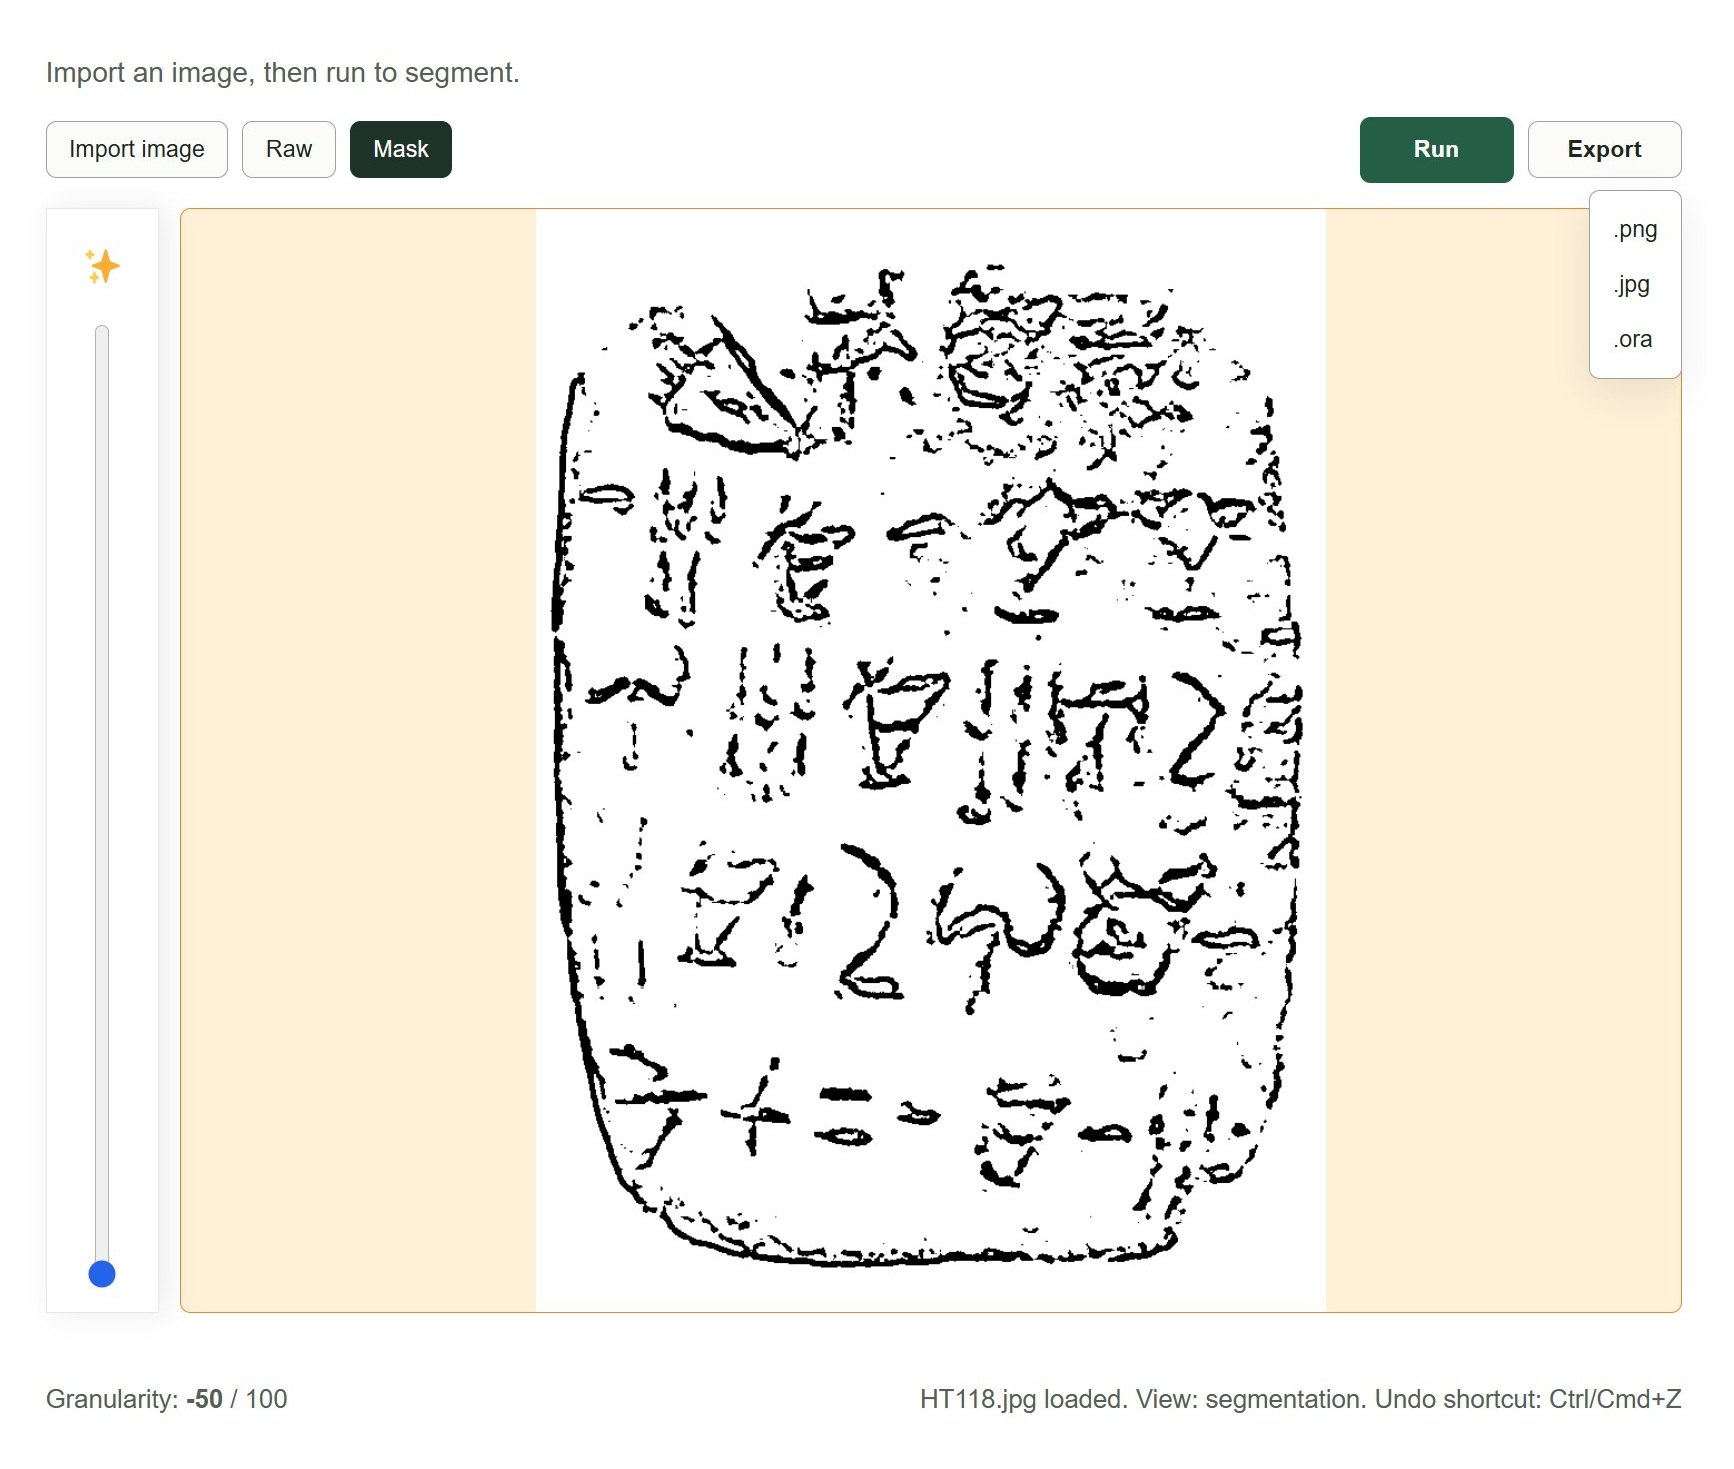
\includegraphics[width=\linewidth]{images/Classic-tool.jpg}}
    \caption{In-tool view of the classical Gaussian adaptive thresholding tool in the mask view.}
    \label{fig:classic_tool}
\end{figure}


\subsubsection{Integration of the classical method}
Chosen to represent classical segmentation methods was the best classical method from the non-interactive evaluation, Gaussian adaptive thresholding (see \cref{Segmentation quality,subsec:classical_comparison}).
On the basis of user feedback during the usability tests (see \cref{appendix:usability-tests}), a slider was added as an interactive way to control the coarseness of the segmentation.
A range of "granularity" was given $[-50,100]$, where 0 represented the default hyperparameters of the model.
The higher the value of this "granularity" slider, the more coarse the segmented mask would turn out, and the lower the value, the more fine-grained it would be.
In that way, the user could adjust the coarseness of the output mask without having to worry about the specific hyperparameters of the model, and without having to understand how they work.
This worked by defining the Gaussian kernel size $D_{\mathrm{Gaussian}}$ as a function of the granularity value as follows (where $g$ is the value of granularity, and $D_{\mathrm{Gaussian,default}}$ denotes the default kernel size of the model):

$$D_{\mathrm{Gaussian}} = \max\left(5,\; D_{\mathrm{Gaussian,default}} + 2\left\lfloor \frac{g}{5} \right\rfloor \right)$$

The granularity value was thus divided by 5 (making the intuitive larger percentage-style range $[-50,100]$ possible), and then rounded down to the nearest integer, to determine how many times the kernel size should be increased by 2 (to keep it odd), with a minimum kernel size of 5 to avoid meaningless too fine-grained outputs.
A view of this method and the granularity slider can be seen in \cref{fig:classic_tool}, where the slider is located in the toolbar on the left.


\subsubsection{Integration of SAM}
Chosen to represent \acs{SAM} was the vanilla version of \acs{SAM}2.
This choice introduced an internal-external selection asymmetry, as the classical method was selected based on the preceding empirical evaluation (\cref{subsec:classical_comparison}), whereas vanilla \acs{SAM}2 was selected on external empirical grounds due to its documented \acs{SOTA} performance in general interactive segmentation \parencite{sam2}.
This was deemed appropriate because the non-interactive evaluation described in the previous section could not determine how \acs{SAM} would perform when used interactively.

It was decided to make full use of its interactive capabilities, including both box prompts, and foreground and background point prompts, as this seemed to be the best way to represent its potential.
But there was one problem.
The mask decoder for \acs{SAM}2 (and \acs{SAM} for that matter) only takes one box prompt at a time, which is not ideal when wanting to segment multiple signs of interest within the same tablet.
To circumvent this, the prompts given to it when boxes were present were processed in the mask decoder so that a separate mask was generated once for each $n$ box prompts placed, also passing only the point prompts within it (see \cref{fig:sam_tool} for the associated user interface).
These $n$ masks were then at last merged together by a pixel-wise logical OR operation to generate the final segmentation mask.

This was still sensible computationally, as predictions were split up such that the image encoder was only executed once on image import, while the mask decoder (as described in \cref{subsubsec:SAM_architecture}) is lightweight enough that it could be executed multiple times without a significant increase in latency.
And even though one strongly oversegmented mask from any single box could inflate the combined result, each predicted mask was expected to remain largely confined to the prompted region due to the nature of box prompts.

Included in the prompt placement interface of the tool was a toolbar consisting of the following tool buttons (see \cref{fig:sam_tool} and \cref{fig:sam_tool_export} for in-tool views of the SAM-based tool, with the toolbar on the left):
\begin{itemize}
    \item \texttt{Box prompt}: When selected, allowed the user to place box prompts on the canvas by clicking the pixel coordinates of the corners that should define the box.
    \item \texttt{Foreground prompt}: When selected, allowed the user to place foreground point prompts on the canvas by clicking on the pixel coordinates they want to include in the segmentation.
    \item \texttt{Background prompt}: When selected, allowed the user to place background point prompts on the canvas by clicking on the pixel coordinates they want to exclude from the segmentation.
    \item \texttt{Eraser}: When selected, allowed the user to remove any placed prompts by clicking on them.
    \item \texttt{Undo}: When selected, allowed the user to undo the last prompt-related action performed.
    \item \texttt{Reset}: When clicked, cleared all prompts from the canvas, allowing the user to start over.
\end{itemize}

\begin{figure}[htp]
    \centering
    \fbox{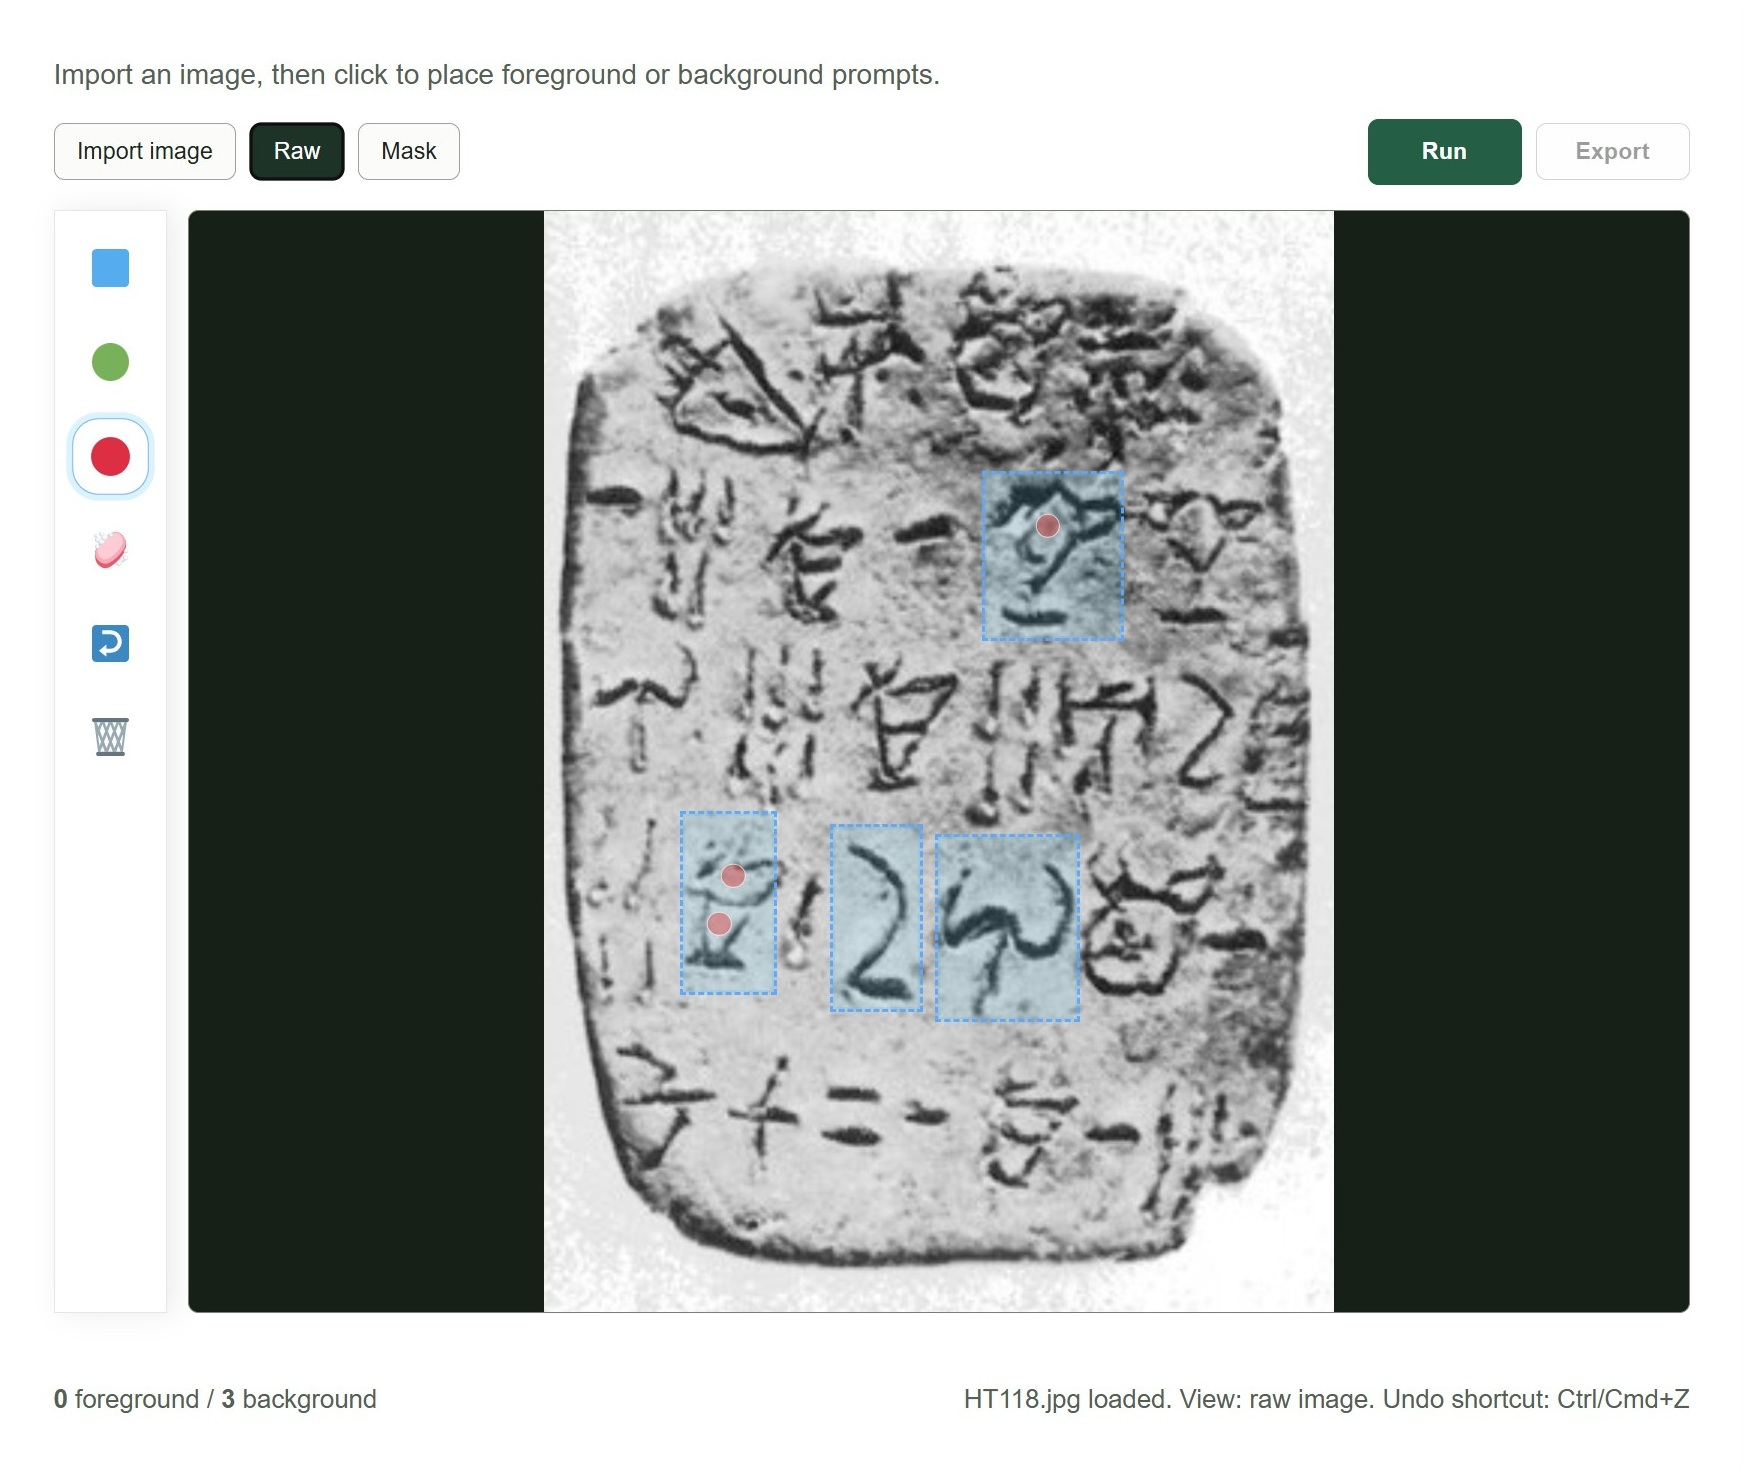
\includegraphics[width=\linewidth]{images/SAM-tool.jpg}}
    \caption{In-tool view of the \acs{SAM}-based tool in the raw view, with box prompts (in blue) placed around some signs of interest, with correcting background point prompts (in red) placed within the oversegmented regions.}
    \label{fig:sam_tool}
\end{figure}


\begin{figure}[htp]
    \centering
    \fbox{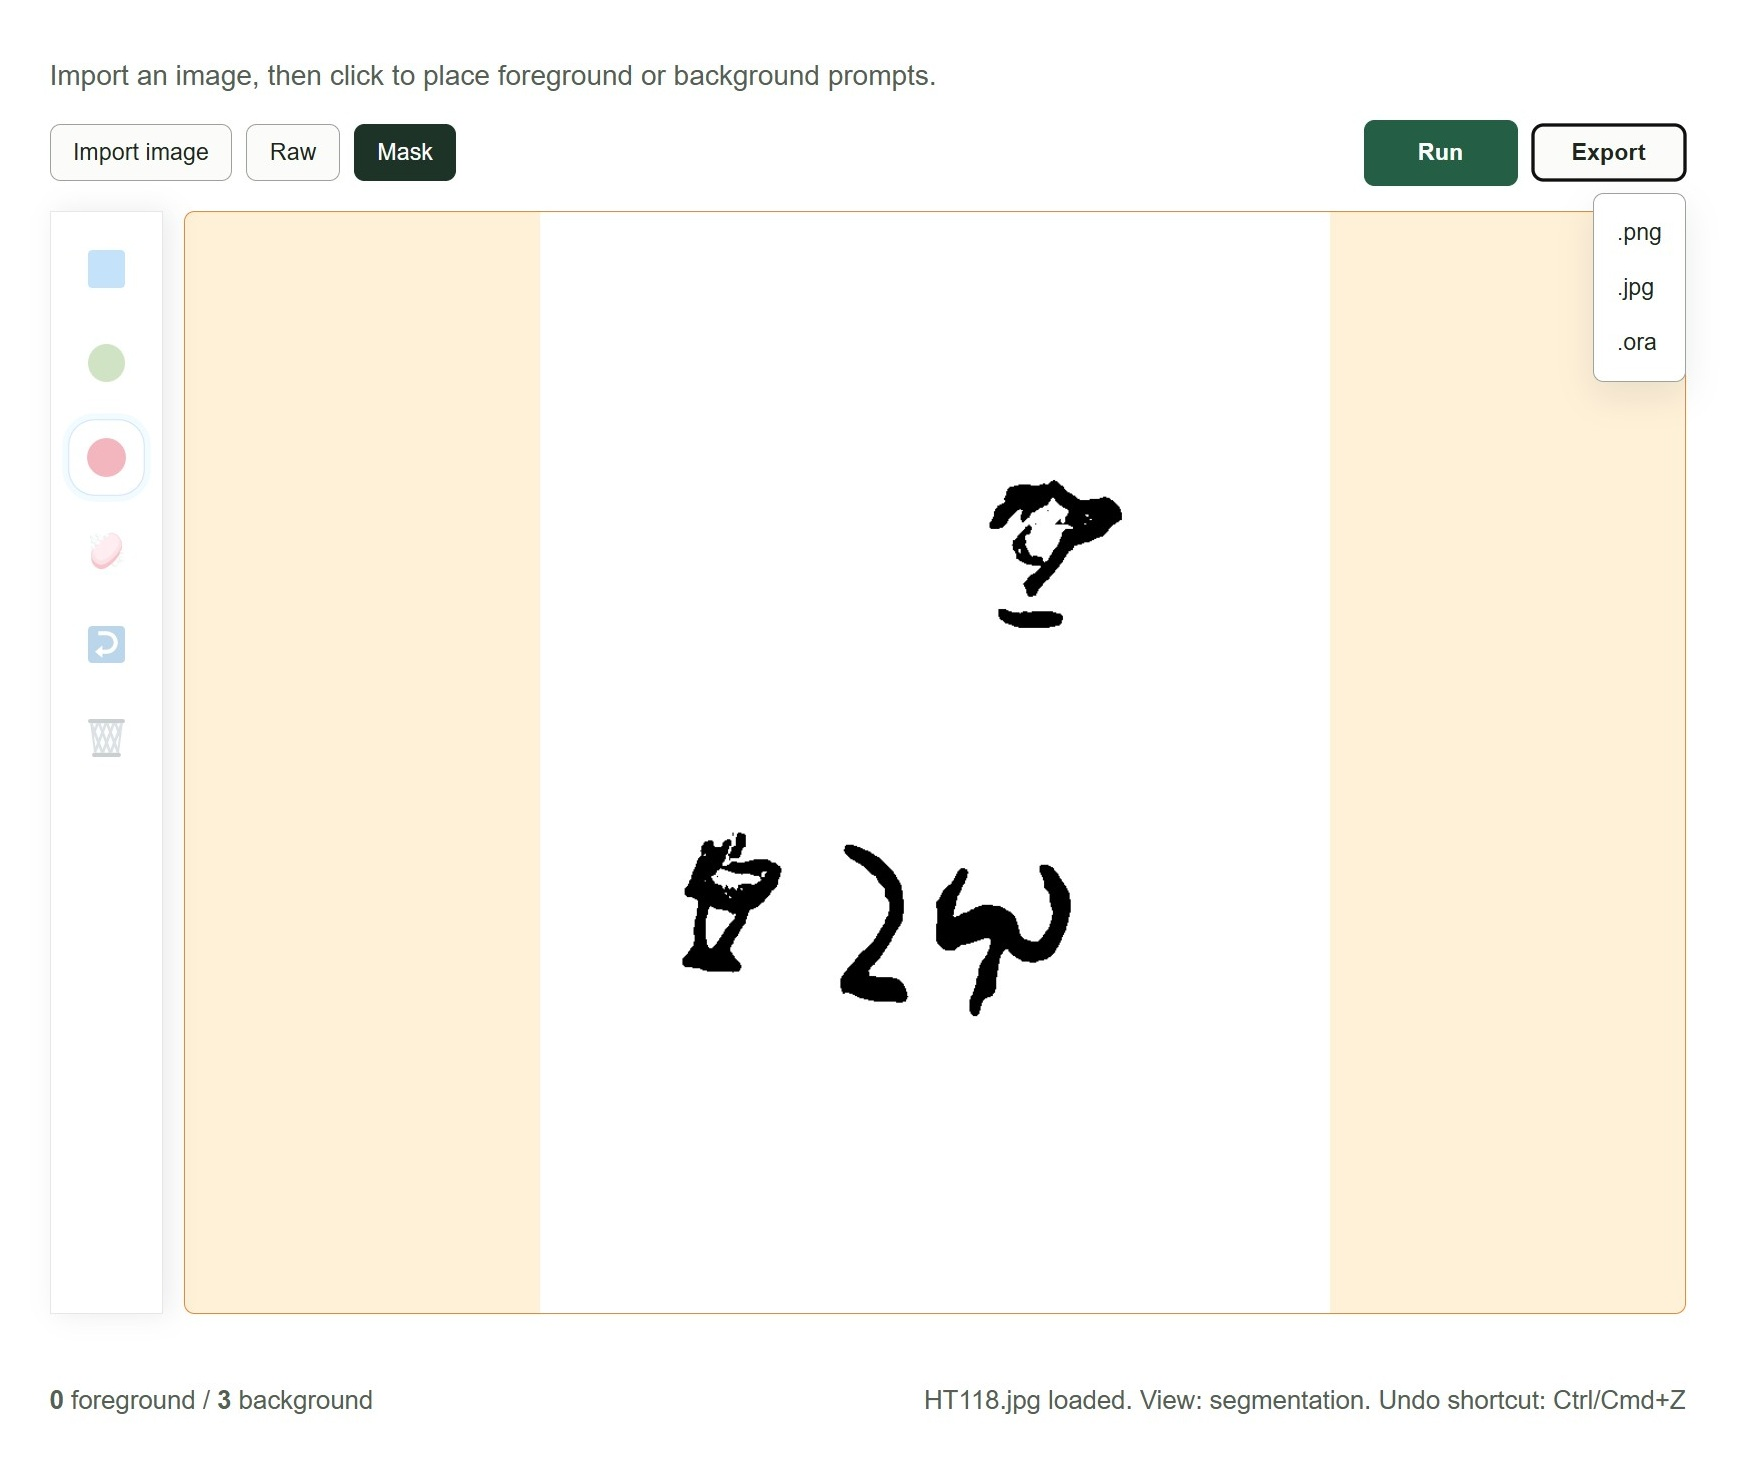
\includegraphics[width=\linewidth]{images/SAM-tool-export.jpg}}
    \caption{In-tool view of the \acs{SAM}-based tool in the mask view, before export of the mask generated from the prompts placed as seen in \cref{fig:sam_tool}.}
    \label{fig:sam_tool_export}
\end{figure}


\subsection{Experimental design for \acs{RQ}2}
\label{subsec:experimental_design_interaction_efficiency}
To evaluate the interaction efficiency of the \acs{SAM}-based tool, a case study was conducted with Ester Salgarella, where she was asked to perform the segmentation of 3 documents from the test set (one from each difficulty category) with each method of the tool.
In a wish to obtain statistical power, an inclusion of all 27 test images was initially preferred, but due to time constraints, only 3 documents made it to the evaluation.
That reduced sample size made the evaluation exploratory and case-study-based rather than statistically powered.
However, it still allowed for a direct comparison of the interaction efficiency of the two tools, using quantitative indicators of both time expenditure (minutes), and the quality of the outputs they generated (\acs{Dice}).
The interaction burden could then further be exploratorily decomposed into the time taken for the models to execute, and for \acs{SAM}-based tool, the amount and types of prompts placed.

The experiment itself was conducted in-person with Ester Salgarella as the participant at \acs{AIAS} on the 12th of May on the same day as the last usability and acceptance test.
Specifically, she was instructed to make use of the tool method evaluated on the document given until she deemed that she could not further improve the segmentation output, whereafter she should export the final mask as it was.
The order of the methods tested was not randomized: the classical tool was tested first, followed by the \acs{SAM}-based tool.
Possible order effects, such as fatigue, are therefore treated as a methodological constraint.
Tool interaction was recorded by the help of live screen recordings via Microsoft Teams, wherefrom the model execution time, the prompts placed, and the time taken from image import to mask export were all measured.
The exports of each tool were also saved on disk, so that \acs{Dice} scores could later be computed therefrom.

\section{Workflow integration} \label{Workflow efficiency}
To answer the question of \hyperref[rq3]{\acs{RQ}3}: \textit{How much reduction in annotation time can be achieved using the proposed tool compared to fully manual digitization, under controlled experimental conditions?}, another case study of 3 documents was conducted with Ester Salgarella, where the time taken to finish polishing the segmentation outputs exported from the two developed tools (see \cref{Interaction efficiency}) was measured, and compared to the time taken to do the same drawings fully manually.

The following subsections go into more details on the workflow definition, the attempt made to fit the tool into it, and the experimental design for the evaluation of this workflow efficiency.

\subsection{Definition of the workflow}
\label{subsection:definition_of_workflow}
The tool was designed to fit into Ester's existing workflow as much as possible, to make it more likely that she would be able to use it with minimal friction, and to make the evaluation of its efficiency more ecologically valid.
To do that, however, it was necessary to first understand her workflow in detail.
\Cref{fig:tool-workflow} illustrates this workflow and where the tool was designed to fit into it, up to the marked \textit{scope cutoff}.

\begin{figure}[htbp]
\centering
\begin{tikzpicture}[
    node distance=1.2cm and 1.4cm,
    tool/.style={
        rectangle,
        rounded corners,
        draw=orange!60!black,
        fill=orange!15,
        align=center,
        minimum width=4.2cm,
        minimum height=0.9cm,
        inner sep=5pt
    },
    interactive/.style={
        rectangle,
        rounded corners,
        draw=blue!60!black,
        fill=blue!15,
        align=center,
        minimum width=4.2cm,
        minimum height=0.9cm,
        inner sep=5pt
    },
    existing/.style={
        rectangle,
        rounded corners,
        draw=green!60!black,
        fill=green!15,
        align=center,
        minimum width=4.2cm,
        minimum height=0.9cm,
        inner sep=5pt
    },
    outside/.style={
        rectangle,
        rounded corners,
        draw=black!55,
        dashed,
        fill=white,
        align=center,
        minimum width=4.2cm,
        minimum height=0.9cm,
        inner sep=5pt
    },
    arrow/.style={-{Latex}, thick},
    looparrow/.style={-{Latex}, thick, dashed},
    optional/.style={-{Latex}, thick, dashed, draw=black!60}
]



\node[tool] (import) {
    Import image\\
    \footnotesize Ctrl+V / file drop / choose file
};

\node[interactive, below= 1.5cm of import] (run) {
    "Run" segmentation
};

\node[interactive, below=of run] (preview) {
    "Mask" preview
};

\node[interactive, right=of run] (adjust) {
    Optional adjustment\\
    \footnotesize prompts / granularity
};

\node[tool, below=of preview] (export) {
    Export\\
    \footnotesize .ora / .png / .jpeg
};

% Existing workflow continues
\node[existing, right=of export] (krita) {
    Open in Krita
};

\node[existing, below=of krita] (finish) {
    Finish drawing
};

\node[outside, below=1.8cm of finish] (layers) {
    Split into layers\\
    \footnotesize add metadata
};

\node[outside, below=of layers] (export-final) {
    Export to JSON\\
};

% Groups


\begin{scope}[on background layer]
\node[
    draw=blue!60!black,
    fill=blue!3,
    rounded corners,
    dashed,
    inner sep=0.35cm,
    fit= (run) (adjust) (preview),
    label={[blue!60!black]above:Iterative interaction}
] (interactivegroup) {};
\end{scope}

\begin{scope}[on background layer]
\node[
    draw=green!60!black,
    fill=green!3,
    rounded corners,
    dashed,
    inner sep=0.35cm,
    fit= (krita) (finish) (layers) (export-final),
] (kritagroup) {};
\end{scope}

\node[
    green!60!black,
    left=0.3cm of kritagroup,
    align=center
] {
    Krita post-editing
};


% Main snake arrows
\draw[optional] (import) -| (adjust);
\draw[arrow] (import) -- (run);
\draw[optional] (adjust) -- (run);
\draw[arrow] (run) -- (preview);
\draw[optional] (preview) -| (adjust);

\draw[arrow] (preview) -- (export);
\draw[arrow] (export) -- (krita);
\draw[arrow] (krita) -- (finish);
\draw[arrow] (finish) -- (layers);
\draw[arrow] (layers) -- (export-final);

\draw[
    dashed,
    thick,
    draw=black!55
]
    ($(finish.south west)+(-0.4,-0.85)$) --
    node[midway, fill=green!3, inner sep=3pt, ] {scope cutoff}
    ($(finish.south east)+(0.4,-0.85)$);



\end{tikzpicture}
\caption{User-facing workflow of the developed segmentation tool and its relation to the existing Krita-based annotation workflow.}
\label{fig:tool-workflow}
\end{figure}

When Ester does the annotation of a document from the \acs{GORILA} corpus, she first imports a screenshot of the \acs{GORILA} corpus drawing into Krita, creating a new layer on top of it to do the segmentation drawing.
She draws this drawing with a digital pen on a displayless pressure-sensitive Wacom drawing pad.
While doing that, she looks for any possible mistakes in the signs, with the original image, and her mental map of the sign types as guidance, correcting them by erasing and redrawing.
At last, when she is satisfied with the drawing, she splits each sign into a separate layer, adds metadata, and imports to SigLA as JSON and Krita files.

Due to scope limitations, it was only the process before that splitting into layers and adding of metadata that this project aimed to improve.
\subsection{The adaptation (export to Krita)}
\label{subsection:export_to_krita}
When the segmentation of a document within the tool was complete, it was designed to allow for export to JPEG, PNG, or OpenRaster (\texttt{.ora}) format.
The latter is an open file format that like Krita (\texttt{.kra}) files consists of a ZIP file with an XML document describing the layer structure, together with a PNG or SVG image for each raster or vector layer, respectively.
This is simpler in structure and easier to read and write for external programs than the \texttt{.kra} file format, since it was specifically designed as an open exchange format between graphics editors.
Krita files, on the other hand, are more complex in structure, including proprietary elements, and not designed for external programmatic access, as they are meant to be used within Krita only.

Additionally, OpenRaster (\texttt{.ora}) format is supported by a few image editing programs, including Krita, which makes it ideal for the exported file to be directly opened there for further manual editing and annotation.
And as Krita was already part of Ester's workflow, it was only natural to make the exported starting point suggestions from the tools directly compatible with it, to make the transition from tool to manual post-editing as seamless as possible.
This file format also made it possible for the tool export to include the original image as a layer, and the generated mask as another, so that the former could be used as a guiding reference for post-editing of the latter.

\subsection{Experimental design for \acs{RQ}3} \label{subsec:experimental_design_workflow_efficiency}
To evaluate the workflow efficiency of the two developed tools (see \cref{Interaction efficiency}), the time it took Ester Salgarella to do the manual annotation workflow in Krita was compared in a case study of 3 documents to the time taken when doing the complete workflow of each of these tools.
The workflow efficiency metric was defined as the sum of tool time (image import to mask export) and drawing time in Krita -- which for the tools was defined by post-editing time (polishing the tool-suggested mask draft until completion).

Thus, this workflow efficiency case study was built upon the tool-related data (of tool time and mask exports) obtained from the in-tool case study (see \cref{Interaction efficiency,subsec:experimental_design_interaction_efficiency}).
Hence, both studies suffered from the same time-constraint-caused limitations in terms of sample size and statistical power, making them exploratory and case-study-based rather than statistically powered.

The drawings in Krita were made using the displayless pressure-sensitive Wacom drawing pad with a pen input used in Ester's original workflow (see \cref{fig:tool-workflow}).
The case study was not done in-person, but consisted of Ester Salgarella remotely post-editing the tool exports from the interaction efficiency study in Krita, recording the time taken on her phone.
For the manual workflow, she was then asked to do the same drawings, but from scratch without any tool-suggested mask draft.
And as a proof of completion, Ester was asked to send the finished \texttt{.ora} files back again.

Even with the originally imported raw tablet images included as layers in the exported \texttt{.ora} files, Ester expressed a lack of guiding reference to know when the drawing was complete.
Therefore, the corresponding \acs{GORILA} corpus expert drawing for each document was manually imported, aligned with the other two layers, and included as an additional layer in the exported \texttt{.ora} file before letting Ester start the post-editing.
For the manual workflow, all of these layers except the tool-suggested draft were also included, to make the comparison as fair as possible.

